\documentclass[a4paper,10pt]{article}
\usepackage[utf8]{inputenc}
\usepackage[toc]{appendix}

\usepackage{geometry}
\usepackage{graphicx}
\usepackage{hyperref}
\usepackage{setspace}
\usepackage{titlesec}

\geometry{a4paper, margin=1in}
\doublespacing
\titleformat{\section}[block]{\normalfont\Large\bfseries}{\thesection}{1em}{}
\titleformat{\subsection}[block]{\normalfont\large\bfseries}{\thesubsection}{1em}{}
\titleformat{\subsubsection}[block]{\normalfont\normalsize\bfseries}{\thesubsubsection}{1em}{}

\begin{document}

\title{Carried away by Long Short-Term Memory: A Machine Learning Approach to Forecasting Carry Trade Returns}
\author{Anton Aleynikov \& Sergey Mirzoev}
\date{\today}
\maketitle

\begin{abstract}

\textbf{Carry trade}, a risky arbitrage strategy exploiting interest rate differentials between two currencies, challenges foreign exchange market efficiency. This research project builds upon the work of Wang et al. (2021) ~\cite{wang2021machine}, which employed long short-term memory (LSTM) networks to forecast carry trade returns. Using a data set spanning 1990 to 2017 for 10 currencies, the study found that LSTM models outperformed traditional linear and threshold regression models based on economic fundamentals. Additionally, the research revealed a deterioration in excess carry trade returns after the 2007–2008 global financial crisis, suggesting a potential impact on the uncovered interest rate parity.
\end{abstract}

\section{Introduction}

% Brief overview of carry trade and its significance in the forex market.
% Introduction to the challenge of persistent excess carry trade returns and its implications for market efficiency.
% Reference to Wang et al. (2021) and their findings using LSTM networks.

Carry trade is a significant phenomenon in the forex market, affecting interest rate differentials, risk-return dynamics, market liquidity, and volume. However, the problem of excess carry trade returns poses a challenge to market efficiency. When carry trade returns exceed what would be expected based on interest rate differentials, it raises questions about the factors driving the extended abnormal returns and challenges the principles of the Efficient Market Hypothesis (\hyperref[appx:emh]{EMH}).

This concern calls for a closer examination of behavioural factors influencing trading decisions. To address this issue, this research builds on the work of Wang et al. (2021) ~\cite{wang2021machine} by using long short-term memory (\hyperref[appx:lstm]{LSTM}) networks to forecast carry trade returns, which is a novel approach compared to traditional models.

This study focuses on existing literature on carry trade and forecasting models, compares LSTM networks with linear and threshold regression models, and delves into the methodology, results, and implications for forex market efficiency and carry trade strategies.

The primary objective of this research is to improve our understanding of carry trade dynamics, with a focus on forecasting models. By comparing the LSTM approach with traditional models, we aim to evaluate the effectiveness of machine learning in predicting carry trade returns and contribute to the body of knowledge on this topic.

\section{Literature Review}
% Explore existing literature on carry trade and forecasting models.
% Discuss traditional models based on economic fundamentals.
% Introduce machine learning approaches, focusing on LSTM networks.

Carry trade, a risky arbitrage strategy based on interest rate differentials between currencies has been the subject of extensive research in financial economics. The returns from carry trades are intricately tied to changes in exchange rates and interest rate differentials across countries. Despite the challenges it poses to the Efficient Market Hypothesis (EMH), there is evidence suggesting that Uncovered Interest Parity (UIP) may hold in the long run, leading to the reversal of excess carry trade returns \cite{wang2021machine}.

\subsection{Excess Carry Trade Returns}

The literature on excess carry trade returns has explored various factors influencing the predictability of these returns. Engel (2014) ~\cite{engel2014exchange} emphasized the importance of introducing nonlinear relationships between explanatory factors, with Jorda and Taylor (2012) ~\cite{jorda2012carry} revealing the effectiveness of incorporating thresholds of fundamentals in improving predictability. Lustig and Verdelhan (2007) ~\cite{lustig2007cross}, as well as Menkhoff et al. (2012) ~\cite{menkhoff2012carry}, highlighted the relevance of volatility in exchange rates and economic fundamentals to carry trade returns.

Furthermore, the aftermath of the 2007–2008 global financial crisis has reshaped the landscape of carry trade returns. With interest rates near zero in the U.S. and other countries, the dominance of exchange rate movements in carry trade returns has increased ~\cite{rossi2013exchange}. The predictability of exchange rates has also been shown to depend on the forecast horizon length, with implications for model specifications ~\cite{chinn2006partial}.

\subsection{Machine Learning Approaches in Carry Trade Prediction}

A significant development in the literature is the integration of machine learning techniques to enhance carry trade return prediction. Gu et al. (2020) ~\cite{gu2020empirical} demonstrated the ability of machine learning to capture nonlinear interactions between predictors, opening new avenues for empirical asset pricing. In particular, the application of Long Short-Term Memory (LSTM) networks, a type of recurrent neural network, has gained prominence for time series forecasting in economic settings \cite{wang2021machine}.

\subsection{Application of LSTM Networks}

This paper contributes to the literature by introducing LSTM networks to predict carry trade returns. LSTM networks, initially developed by Hochreiter and Schmidhuber (1997), have the unique ability to memorize long-term data patterns, optimizing explanatory factors and data length. The analysis is conducted on a monthly dataset spanning G10 currencies between 1990 and 2017, revealing that LSTM networks outperform traditional models regarding average return, Sharpe ratio, and gain/loss ratio.

\subsection{Post-Crisis Carry Trade Returns}

The findings of this paper indicate a deterioration in carry trade returns after the 2007–2008 global financial crisis, consistent with the trend observed in interest rate differentials shrinking to near zero \cite{accominotti2019currency}. This provides supportive evidence that excess carry trade returns may be influenced by long-term changes in interest rate differentials, aligning with the UIP hypothesis.

\subsection{Comparison and Contribution}

In comparison with commonly used models such as random walk, vector autoregression (VAR), threshold vector error correction model (TECM), and traditional recurrent neural networks (RNN), LSTM networks demonstrate superior performance in forecasting carry trade returns. The results contribute to the literature by showcasing the potential of LSTM networks to improve predictability and reduce risk in carry trade portfolios \cite{davis2020economic}.

Future research may explore the applicability of LSTM networks in other economic settings and further investigate the nuanced features of carry trade returns, especially in the context of evolving market conditions post-financial crisis.


\section{Methodology}

In this section, we detail the methodology employed in forecasting carry trade returns, covering the dataset, the currencies involved, and the period under consideration. Additionally, we comprehensively compare the Long Short-Term Memory (LSTM) approach and traditional linear and threshold regression models.

\subsection{Dataset}

The dataset used in this study spans from 1990 to 2017 and includes monthly data for 10 major currencies. These currencies are the focal point of our analysis, with exchange rate and one-month risk-free interest rate data sourced from Datastream. The consumer price index data for G10 countries is sourced from FRED Economic Data to capture the inflation dynamics. It's important to note that all assessed countries operate under a floating exchange rate regime and allow free capital mobility.

\subsection{Carry Trade Return Estimation}

Following the methodology proposed by Jordan and Taylor (2012), we estimate carry trade returns using a framework with the U.S. as the home country in a currency pair. The ex-post nominal excess return for a carry trade at time \(t+1\) is defined as:
\[ s_{t+1} = \Delta e_{t+1} + (i^*_t - i_t) \]
where \(\Delta e_{t+1}\) is the logged exchange rate difference, and \(i^*_t\) and \(i_t\) are the foreign and home one-period, risk-free interest rates, respectively.

To further analyse carry trade returns in real terms, we introduce the real exchange rate \(q_{t+1}\):
\[ q_{t+1} = \bar{q} + e_{t+1} + (p^*_{t+1} - p_{t+1}) \]
Under the assumption of purchasing power parity (PPP), the real exchange rate \(q_t\) converges to \(\bar{q}\), and \(q_t - \bar{q}\) is stationary. The carry trade return in real terms (\(s_{t+1}\)) can be expressed as:
\[ s_{t+1} = \Delta q_{t+1} + (r^*_t - r_t) \]
where \(\Delta q_{t+1}\) is the stationary component of the real exchange rate difference, and \(r^*_t\) and \(r_t\) are the foreign and home real interest rates.

\subsection{Forecasting Models}

We employ \hyperref[appx:lstm]{LSTM} networks, a recurrent neural network (\hyperref[appx:rnn]{RNN}), for carry trade return forecasting. The LSTM networks incorporate memory cells and gating mechanisms, enabling them to capture long-term dependencies in the data.

For comparison, we consider traditional linear models such as the random walk, vector auto-regression (\hyperref[appx:var]{VAR}), and the threshold vector error correction model (\hyperref[appx:tecm]{TECM}). Additionally, we include a degenerated RNN model by shutting down the memory cell gate structure to assess the impact of memory cells in the LSTM architecture.

\subsection{Model Comparison}

To assess the performance of the forecasting models, we conduct a thorough comparison based on various metrics, including mean returns, standard deviations, skewness, kurtosis, Sharpe ratios, gain/loss ratios, Diebold-Mariano tests, and out-of-sample \(R^2\). The comparison spans three rolling windows: 2012–2015, 2013–2016, and 2014–2017.

This detailed analysis aims to provide insights into the effectiveness of the LSTM approach compared to traditional linear and threshold regression models in forecasting carry trade returns over the specified period.


\section{Results}

\subsection{Exchange Rate Predictions}

In this section, we present the predictions of our models for the exchange rates of G10 currencies without the US. Figure \ref{fig:lstm_predictions} shows the LSTM model's predictions, and Figure \ref{fig:rnn_predictions} displays the RNN model's predictions.

\begin{figure}[ht]
    \centering
    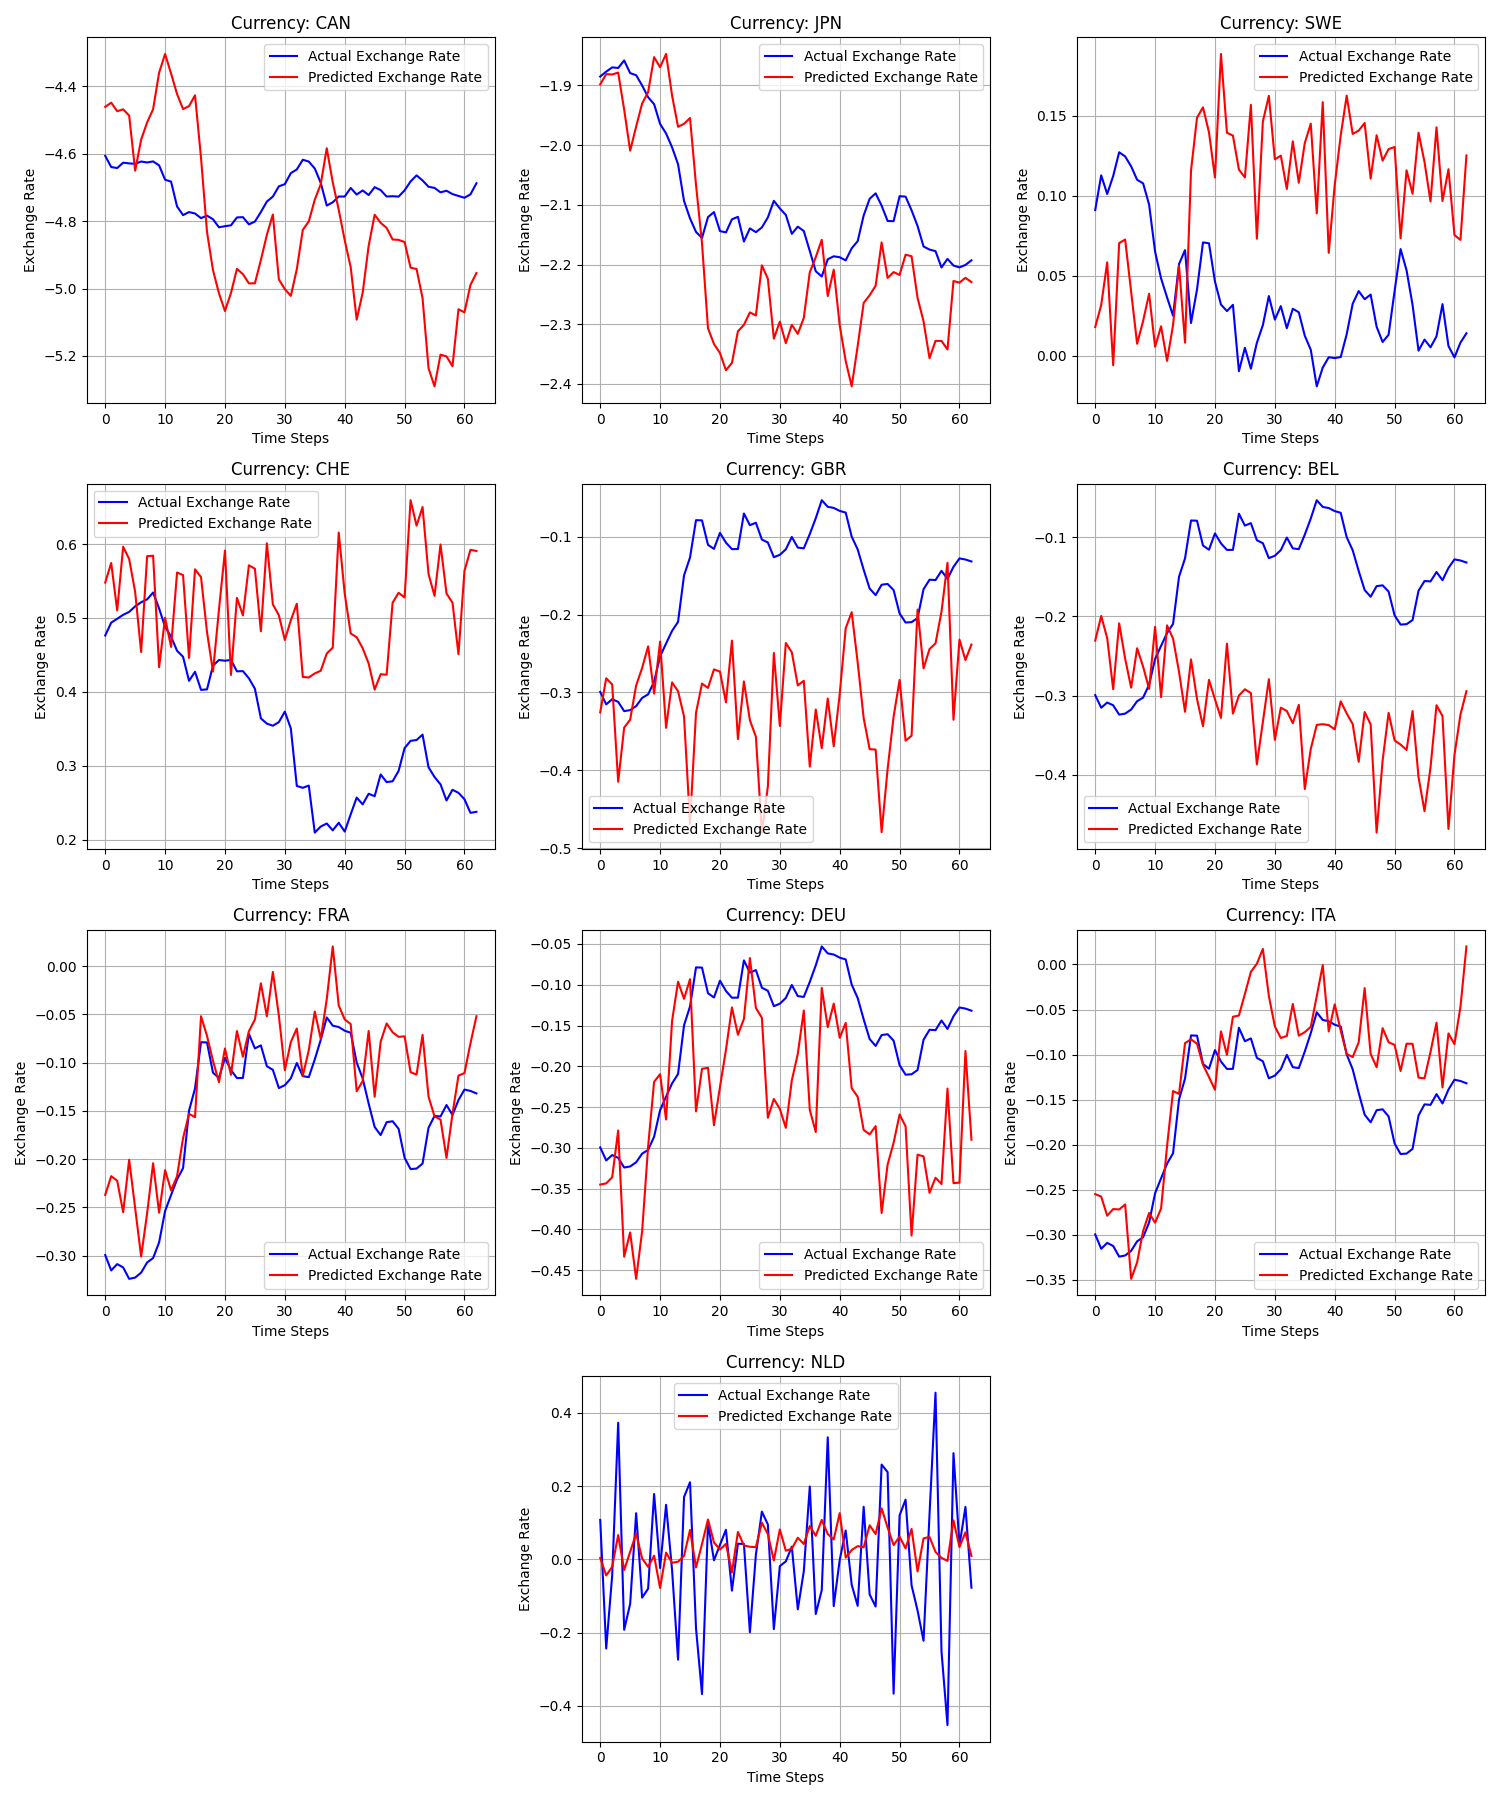
\includegraphics[width=0.8\textwidth]{fig/lstm_exchange_rate_predictions.png}
    \caption{LSTM Exchange Rate Predictions}
    \label{fig:lstm_predictions}
\end{figure}

\begin{figure}[ht]
    \centering
    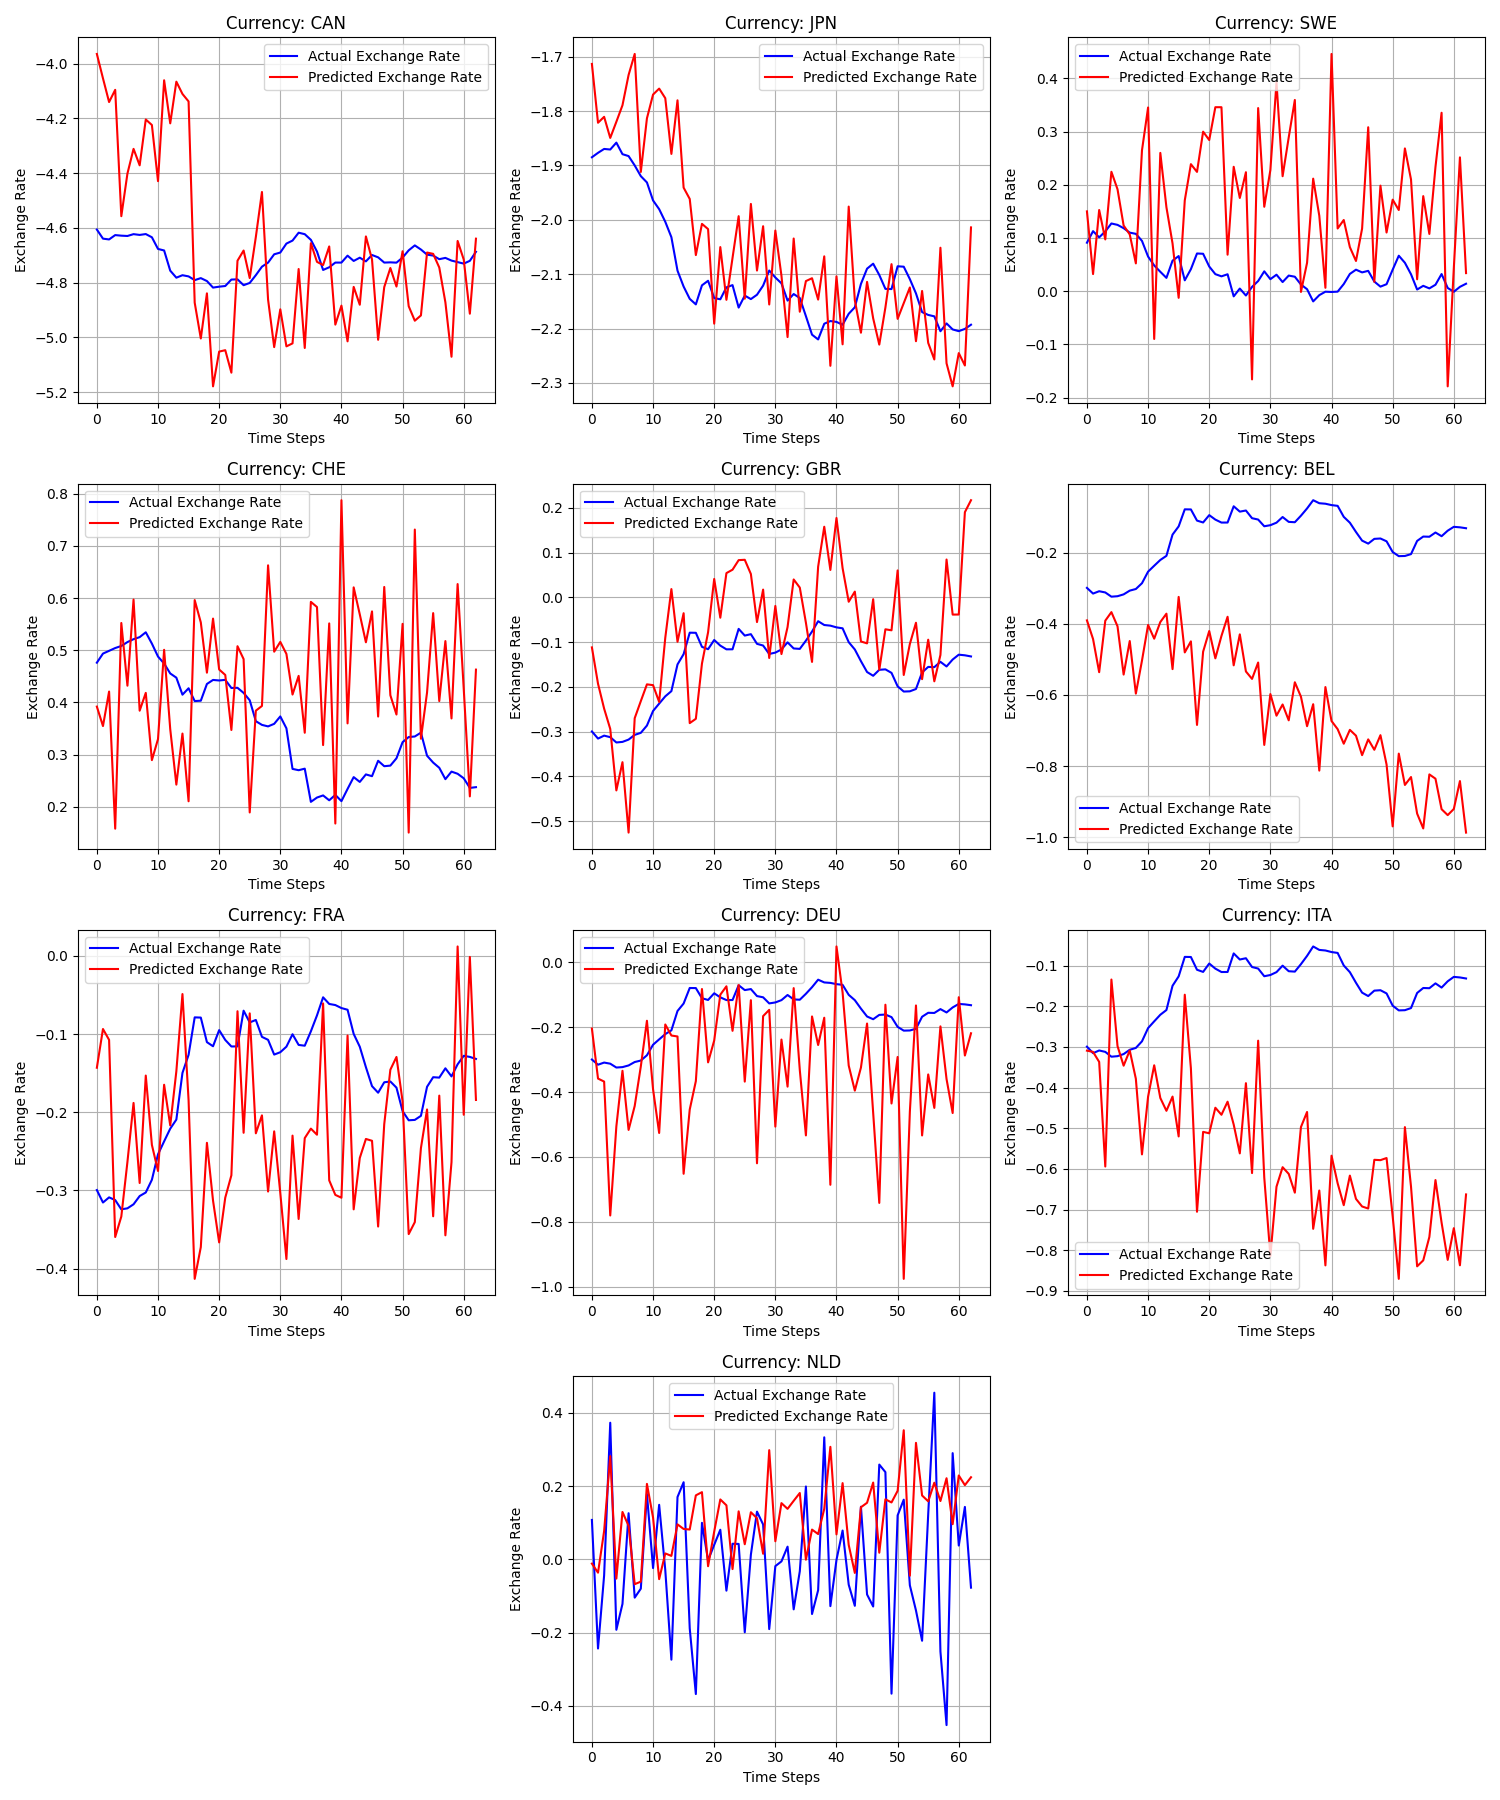
\includegraphics[width=0.8\textwidth]{fig/rnn_exchange_rate_predictions.png}
    \caption{RNN Exchange Rate Predictions}
    \label{fig:rnn_predictions}
\end{figure}

As observed in the figures, the LSTM model generally performed well in estimating the level and capturing the long-term trend of the time series as well as short-term changes. However, it struggled with sudden jumps, failing to accurately predict these abrupt changes. On the other hand, the RNN model exhibited challenges in capturing both the long-term trend and short-term fluctuations, with notable difficulties in predicting jumps.



\subsection{Wang}

Present the results of the LSTM model in forecasting carry trade returns.
Compare these results with the findings of Wang et al. (2021) ~\cite{wang2021machine}.
Highlight any significant differences or improvements observed with LSTM.

\section{Discussion}

The limitations in predicting jumps in both machine learning models may suggest that additional data could enhance the models' performance. Apart from the features used, such as 'Log-nominal exchange rate', 'Real Change to 12-M Average exchange rate', 'Inflation' and 'Interest Rate,' incorporating monthly realised volatility for each currency might have provided valuable information to help both RNN and LSTM models better capture abrupt changes in exchange rates.

Interpret the results and discuss the implications for carry trade strategies.
Address the deterioration in excess carry trade returns post the 2007–2008 global financial crisis.
Consider the potential implications for uncovered interest rate parity in the long run.

\section{Conclusion}
Summarise the key findings of the research.
Discuss the broader implications for forex market efficiency and carry trade strategies.
Suggest avenues for future research in this area.

% Specify the bibliography style and file
\bibliographystyle{unsrt}
\bibliography{references}

\appendix

\section{ML Foundations}

\subsection{Long Short-Term Memory (LSTM)}\label{appx:lstm}

Long Short-Term Memory (LSTM) is an example of a recurrent neural network (\hyperref[appx:rnn]{RNN}) architecture designed to overcome the vanishing gradient problem associated with traditional RNNs. LSTMs are particularly well-suited for sequence prediction tasks, making them popular in various fields, including time series forecasting and natural language processing.

LSTMs incorporate memory cells and gating mechanisms, allowing them to capture long-term dependencies in sequential data. The fundamental components of an LSTM include the input gate, forget gate, memory cell, and output gate. These gates regulate the flow of information within the LSTM, enabling it to retain or discard information over time selectively.

The information flow within an LSTM can be outlined as follows:

\begin{enumerate}
  \item \textbf{Forget Gate:} Determines how much of the previous cell state should be retained and how much should be forgotten.

  \item \textbf{Input Gate:} Controls the amount of new information that should be added to the cell state.

  \item \textbf{Memory Cell:} Stores and updates information based on the input and previous cell state.

  \item \textbf{Output Gate:} Determines the next hidden state based on the current input and cell state.

\end{enumerate}

Figure \ref{fig:lstm_structure} illustrates an LSTM network's structure, showcasing the information flow through the gates and the memory cell.

\begin{figure}[ht]
  \centering
  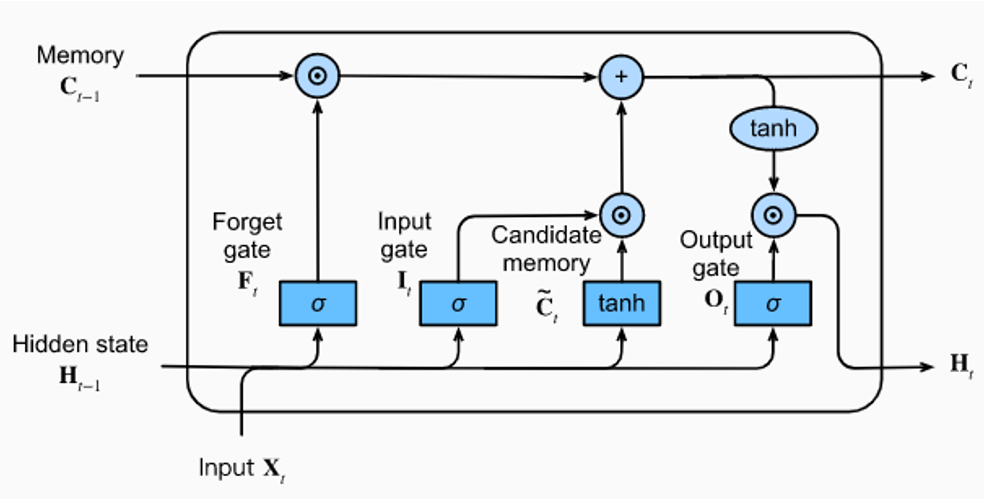
\includegraphics[width=0.8\textwidth]{fig/lstm.png}
  \caption{Structure of a Long Short-Term Memory (LSTM) Network}
  \label{fig:lstm_structure}
\end{figure}

LSTMs have demonstrated superior performance in capturing complex patterns and dependencies in sequential data, making them valuable in various machine-learning applications.

% \clearpage  % Ensure the figure and content appear on the same page

\subsection{Recurrent Neural Network (RNN)}\label{appx:rnn}

Recurrent Neural Networks (RNNs) are designed for sequential data processing and capture dependencies and patterns across time. They have connections that form directed cycles, allowing them to maintain a hidden state that stores information about previous inputs. However, traditional RNNs suffer from the vanishing gradient problem, which limits their ability to capture long-term dependencies. More advanced architectures like Long Short-Term Memory (\hyperref[appx:lstm]{LSTM}) networks have been developed to overcome this limitation.

\section{Economic Foundations}

\subsection{Efficient Market Hypothesis (EMH)}\label{appx:emh}

The Efficient Market Hypothesis (EMH) is a fundamental concept in financial economics that posits that financial markets efficiently incorporate and reflect all relevant information. According to EMH, it is not possible for an investor to consistently achieve higher-than-average returns through the analysis of historical price movements or publicly available information. The hypothesis suggests that asset prices fully reflect all available information, making it impossible to achieve consistent profits by exploiting market inefficiencies.

EMH is typically categorized into three forms:

\begin{enumerate}
  \item \textbf{Weak Form EMH:} Assumes that past price and volume information is already incorporated into current stock prices. Therefore, technical analysis relying on historical price movements would not provide an advantage.

  \item \textbf{Semi-Strong Form EMH:} Posits that all publicly available information is already reflected in stock prices. Consequently, neither fundamental analysis (examining financial statements) nor technical analysis can consistently outperform the market.

  \item \textbf{Strong Form EMH:} Asserts that all public or private information is fully reflected in asset prices. This implies that even insider information cannot be used to achieve superior returns consistently.
\end{enumerate}

EMH has important implications for investors, as it challenges the effectiveness of active trading strategies and supports the notion that a passive buy-and-hold approach may be just as practical in the long run.

\subsection{Uncovered Interest Parity (UIP)}\label{appx:uip}

Uncovered Interest Parity (UIP) is an economic theory in international finance that explores the relationship between interest rates and exchange rates. UIP posits that the expected change in the exchange rate between two currencies is equal to the difference in their nominal interest rates. In other words, when investors do not hedge their currency exposure, they should expect to earn the same return on investment in any currency, regardless of the level of interest rates.

Mathematically, UIP can be expressed as: $ \mathbf{E}(e_{t+1}) = i_t - i^*_t $, where \( \mathbf{E}(e_{t+1}) \) is the expected change in the exchange, \( i_t \) is the domestic interest rate and \( i^*_t \) is the foreign interest rate.

If UIP holds, investors should not be able to profit consistently from differences in interest rates across currencies. However, empirical studies have shown mixed evidence regarding the validity of UIP, with various factors influencing the observed relationship between interest rates and exchange rates.

\subsection{VAR model}\label{appx:var}

The VAR model extends a classical univariate model to a multivariate case by framing the considered set of variables into vectors. Following the original paper, the VAR with lag equal to 1 and the respective variable vector $y_t = [\Delta e_t, \pi^{*}_t - \pi_t, i^{*}_t - i_t, q_t - \bar{q}]^t$ has the following specification:

\begin{equation}
    y_t = Ay_{t-1} + \epsilon_t
\end{equation}

where A is a time-invariant ($4 \times 4$) coefficients matrix, $\epsilon_t$ - zero-mean i.i.d. ($4 \times 1$) error vector with a fixed covariance matrix. 

Note that this specification is vulnerable to the autocorrelatedness of the variables. Thus, the estimation can only be performed on the differenced series, as in our case. The series is also assumed to be stationary. The coefficient matrix captures the cross relationships between the variables through the off-diagonal terms.

\subsection{TVECM}\label{appx:tvecm}

TVECM is an extension of the error correction version of the VAR model. Before addressing the threshold VECM, we describe the classical VECM. 

Keeping our vector of variables $y_t$, the vector autoregressive model with error correction term (VECM) and lag equal 1 has the following specification:

\begin{equation}
\Delta y_t = \Pi y_{t-1} + \Gamma\Delta y_{t-1} + \epsilon_t 
\end{equation}

where $\epsilon_t$ are zero-mean, independent error terms. The model assumes that each series is integrated of order one, i.e. $y_{it}$ ~ $I(1), i = 1, ... , 4$. Under this assumption of cointegration, we can find a stationary linear combination of  $y_{it}$, i.e. $\beta^t y_{it}$ ~ $I(0)$. Thus (2) can be rewritten according as 

\begin{equation}
\Delta y_t = \alpha\beta^ty_{t-1} + \Gamma\Delta y_{t-1} + \epsilon_t 
\end{equation}

where $\beta$ is a $1 \times 4$ vector of cointegration vector and $\alpha$ is a $4 \times 1$ loading vector. The impact of lagged values of $X_{it}$ are characterised by $\Gamma_i$, $i = 1,...,k$ $4 \times 4$ matrix. Note that here, we follow the suggestion of the original paper that assumes a unique cointegrating relationship with $q_t - \bar{q}$ being the cointegrating variable. Thus, the $\beta$ and $\alpha$ are treated as vectors, even though generally, they represent matrices with size dependent on the number of cointegrating relationships. 

In essence, VECM is a model that implies the existence of a long-run stationary relationship between the variables determined by the cointegrating vector while at the same time allowing for short-run deviations from the stationary path described by the $\Gamma$ matrix. The threshold version of VECM assumes multiple stationary regimes for the same stationary long-run path, thus allowing for non-linear long-run relation modelling. We follow the original paper methodology, assuming the presence of 2 regimes. 

\end{document}
